\section{REALab: встроенная перспектива на вмешательство}

\subsection{Ключевые идеи}

Основная идея статьи~\cite{kumar2020realab} заключается в моделировании вмешательства 
в задачах обучения с подкреплением с помощью платформы REALab, которая 
обеспечивает \emph{встроенную} обратную связь посредством физических регистров. 
В отличие от стандартных симуляторов, REALab не использует защищённый канал 
награды: вся обратная связь хранится в объектах среды, которые могут быть 
изменены агентом.

Платформа служит:
\begin{itemize}
    \item инструментом для формального моделирования небезопасных механизмов обратной связи;
    \item тестовой средой для проверки устойчивости алгоритмов к вмешательству;
    \item операционализацией формализма CFMDP в реальной симуляции.
\end{itemize}

\subsection{Математическое описание метода}

Математическая структура задачи задаётся через марковский процесс принятия решений 
с искажённой обратной связью. Взаимодействие между агентом и средой происходит следующим образом:
\begin{equation}
\begin{aligned}
A_t &\in A, \\
K_t &\in K, \\
D_{t+1} &= \delta(S_t, K_t), \\
\tilde{D}_{t+1} &= c(S_{t+1}, K_t, D_{t+1}), \\
S_{t+1} &\sim f(S_t, A_t),
\end{aligned}
\end{equation}
где $\delta$~-- функция обратной связи, определяемая разработчиком агента, а функция $c$ моделируется физикой симуляции.

Истинный возврат определяется как:
\begin{equation}
G = \sum_{t=0}^{T} \gamma^t r(S_t, A_t),
\end{equation}
и не наблюдается агентом.


\subsection{Алгоритм}

REALab не задаёт фиксированный алгоритм обучения: вместо этого платформа
определяет структуру взаимодействия между агентом и встроенными механизмами 
обратной связи. Алгоритм формируется разработчиком агента, который выбирает, 
каким образом использовать влияющие компоненты среды, и включает следующие шаги:

\begin{enumerate}
    \item \emph{Конфигурирование компонентов обратной связи.}
    Разработчик агента выбирает типы регистров, их расположение и необходимые 
    метры. Эти компоненты определяют канал обратной связи, который физически 
    присутствует в среде и подвержен вмешательству.

    \item \emph{Определение функции обратной связи~$\delta$.}
    Поставщик обратной связи получает наблюдения среды и (при необходимости) 
    значения метров, после чего записывает вычисленное значение в выбранные 
    регистры. Эта функция определяет, какие сигналы будут доступны агенту 
    для обучения.

    \item \emph{Выбор алгоритма обучения.}
    Разработчик выбирает способ использования сигналов, поступающих через 
    регистры: обучение по мгновенной награде, поведенческое клонирование, 
    обучение по советам по ценности и т.~д. Платформа не ограничивает выбор 
    метода: она лишь предоставляет механизм доставки обучающих сигналов.

    \item \emph{Взаимодействие в ходе эпизода.}
    На каждом шаге агент получает наблюдение, формирует запрос $K_t$ к 
    поставщику обратной связи, выполняет действие $A_t$, после чего считывает 
    значения из регистров. Записанное значение может отличаться от прочитанного 
    вследствие физической динамики среды, что позволяет исследовать возникновение 
    вмешательства.
\end{enumerate}

Структура ролей проектировщика среды и проектировщика агента, а также 
их взаимодействие с симуляцией, показаны на 
Рисунке~\ref{fig:realab_roles}.

\begin{figure}[h]
    \centering
    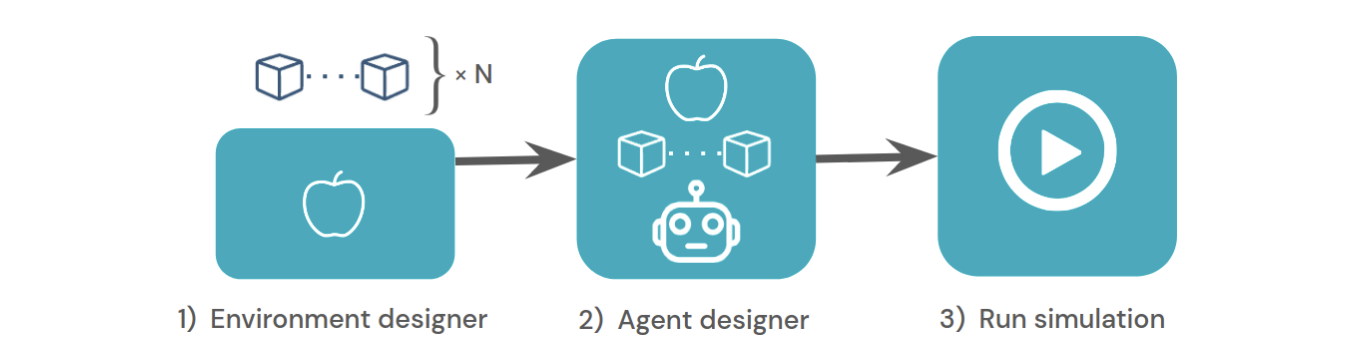
\includegraphics[width=0.9\linewidth]{images/realab_roles.png}
    \caption{Роли проектировщика среды и проектировщика агента в REALab. 
    Проектировщик среды определяет задачу, динамику и доступные компоненты; 
    проектировщик агента конструирует механизм обратной связи и алгоритм обучения;
    симулятор запускает обучение агента, который взаимодействует с компонентами 
    среды и получает наблюдаемую, потенциально повреждённую обратную связь.}
    \label{fig:realab_roles}
\end{figure}

\subsection{Наборы данных}

В платформе REALab отсутствуют заранее подготовленные датасеты: обучение 
и оценка происходят непосредственно в трёхмерной симуляции. Такой формат 
позволяет изучать влияние действий агента на механизм обратной связи, 
поскольку все данные формируются динамически в процессе взаимодействия 
со средой. Источниками данных в REALab выступают:

\begin{itemize}
    \item трёхмерные задачи на игровом движке Unity \cite{unity2018engine};
    \item задания, аналогичные средам DMLab-30 \cite{beattie2016deepmindlab}, 
    например \emph{сбор яблок} или \emph{открытие двери};
    \item компоненты среды (регистры, метры, поставщики обратной связи), 
    которые создают обучающие сигналы во время взаимодействия агента 
    с миром.
\end{itemize}

На Рисунке~\ref{fig:realab_registers} приведён пример сцены в одной из задач: 
объект, предоставляющий награду, и \emph{двухблочный регистр}, значение которого 
кодируется относительным положением блоков.

\begin{figure}[h]
    \centering
    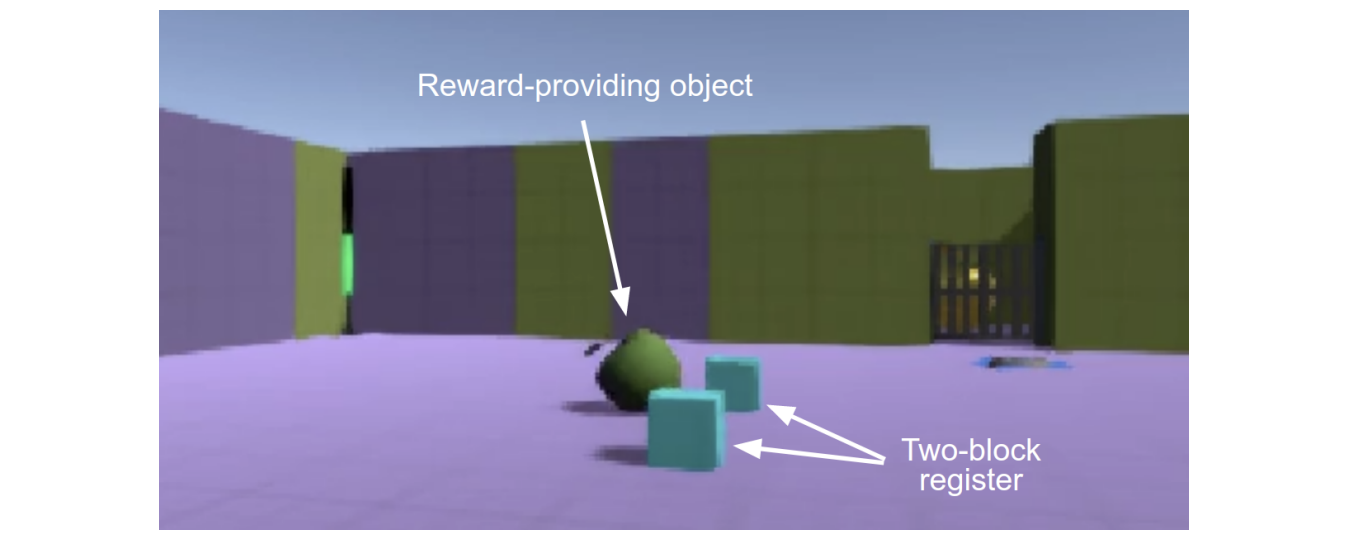
\includegraphics[width=0.9\linewidth]{images/realab_registers.png}
    \caption{Пример сцены в REALab: объект, обеспечивающий награду, и 
    двухблочный регистр, хранящий значение обратной связи. Изменение положения 
    блоков приводит к изменению закодированного значения, что моделирует 
    вмешательство в механизм обратной связи.}
    \label{fig:realab_registers}
\end{figure}

\subsection{Метрики}

Для оценки поведения агента используются метрики, которые отражают два ключевых 
аспекта: соответствие поведения агента истинным задачам среды и наличие или 
отсутствие стимулов к вмешательству.

\begin{itemize}

    \item \emph{Истинный возврат} ~-- основная метрика качества решения задачи.
    Она измеряет, насколько эффективно агент выполняет задание в соответствии 
    с истинной функцией вознаграждения среды (которую он никогда напрямую не 
    наблюдает). Истинный возврат определяется как сумма дисконтированных 
    истинных наград:
    \begin{equation}
        G = \sum_{t=0}^{T} \gamma^t r(S_t, A_t).
    \end{equation}
    Высокое значение $G$ означает, что поведение агента действительно полезно 
    в заданном мире, а не только по наблюдаемой обратной связи.

    \item \emph{Коррупция регистра} ~-- метрика, отражающая степень вмешательства 
    агента в каналы обратной связи. В REALab запись значения обратной связи 
    происходит через физические регистры, которые агент может непреднамеренно 
    или намеренно изменять. Коррупция измеряется как абсолютная разница между 
    значением, записанным поставщиком обратной связи, и тем значением, которое 
    затем считывает агент:
    \begin{equation}
        C = \left| D^\text{write} - D^\text{read} \right|,
    \end{equation}
    где $D^\text{write}$~-- значение, которое поставщик обратной связи отправил 
    в регистр, а $D^\text{read}$~-- значение, которое агент прочитал после 
    физической эволюции среды.
    
    Значение $C>0$ указывает на то, что агент изменил регистр либо напрямую, 
    либо косвенно.

    \item \emph{Сравнение агентов по двумерному показателю} ~-- метрика,
    позволяющая одновременно учитывать полезность поведения и уровень вмешательства. 
    Для каждого агента вычисляется пара значений
    \begin{equation}
        (\text{истинный возврат},\; \text{уровень коррупции}),
    \end{equation}
    что позволяет сравнивать различные архитектуры не только по успешности 
    выполнения задания, но и по тому, насколько они склонны к вэйрхедингу или 
    другим формам вмешательства.
\end{itemize}


\subsection{Модели}

REALab позволяет исследовать различные механизмы обучения, отличающиеся тем, 
как агент получает обратную связь через физические, подверженные вмешательству 
регистры. Ниже приведены три класса моделей, используемых в статье.

\begin{itemize}

    \item \emph{Агент с мгновенной наградой}~\cite{sutton1998reinforcement}.  
    Поставщик обратной связи считывает текущее изменение счёта через метр 
    и записывает его в регистр. Агент воспринимает записанное значение как 
    награду. Поскольку регистр является физическим объектом, изменение его 
    положения или столкновения с ним приводят к искажению наблюдаемой награды.

    \item \emph{Агент имитационного обучения}~\cite{ross2011dagger}.  
    Поставщик обратной связи вычисляет действие демонстратора по текущему 
    наблюдению и записывает его в регистр. Агент обучается повторять эти действия. 
    Такая модель позволяет изучить, может ли агент стремиться менять регистр 
    для упрощения демонстраций.

    \item \emph{Агент, использующий советы по ценности}~\cite{knox2008tamer,daswani2014qadvice}.  
    Поставщик обратной связи вычисляет значение $Q(o,a)$ для наблюдения и выбранного 
    действия, после чего записывает его в регистр. Агент стремится максимизировать 
    наблюдаемое значение совета, что создаёт сильные стимулы к вмешательству 
    в регистр, поскольку изменение его положения напрямую влияет на получаемую оценку.
\end{itemize}

Поведение агентов, использующих советы по ценности, иллюстрируется 
на Рисунке~\ref{fig:realab_valueadvice}: когда агент оказывается рядом с регистром, 
он может переключиться с выполнения задачи на изменение положения регистра, 
повышая наблюдаемую полезность.

\begin{figure}[h]
    \centering
    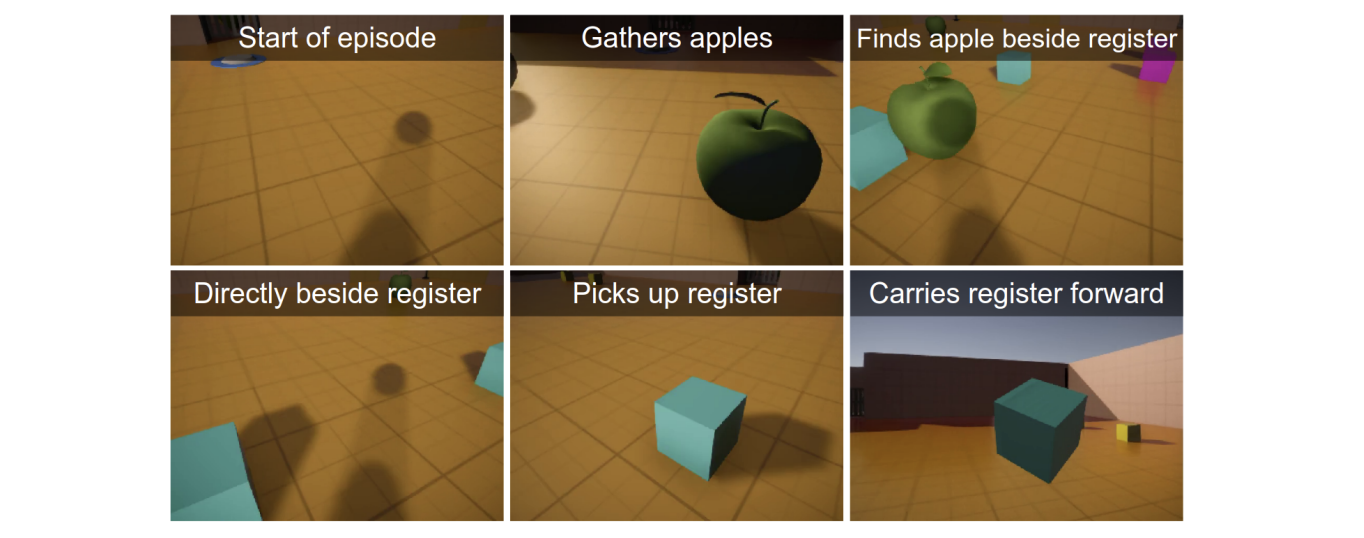
\includegraphics[width=0.95\linewidth]{images/realab_valueadvice.png}
    \caption{Поведение агента, использующего советы по ценности: 
    при возможности агент начинает изменять положение регистра, чтобы 
    повысить наблюдаемое значение обратной связи, вместо выполнения 
    исходной задачи.}
    \label{fig:realab_valueadvice}
\end{figure}

Каждая модель определяется выбором поставщика обратной связи:
\begin{itemize}
    \item приращение счёта;
    \item действие демонстратора;
    \item значение $Q(o,a)$.
\end{itemize}
